%%%%%%%%%%%%%%%%%%%%%%%%%%%%%%%%%%%%%%%%%
% University/School Laboratory Report
% LaTeX Template
% Version 3.1 (25/3/14)
%
% This template has been downloaded from:
% http://www.LaTeXTemplates.com
%
% Original author:
% Linux and Unix Users Group at Virginia Tech Wiki 
% (https://vtluug.org/wiki/Example_LaTeX_chem_lab_report)
%
% License:
% CC BY-NC-SA 3.0 (http://creativecommons.org/licenses/by-nc-sa/3.0/)
%
%%%%%%%%%%%%%%%%%%%%%%%%%%%%%%%%%%%%%%%%%

%----------------------------------------------------------------------------------------
%	PACKAGES AND DOCUMENT CONFIGURATIONS
%----------------------------------------------------------------------------------------

\documentclass{article}

\usepackage[version=3]{mhchem} % Package for chemical equation typesetting
\usepackage{siunitx} % Provides the \SI{}{} and \si{} command for typesetting SI units
\usepackage{graphicx} % Required for the inclusion of images
\usepackage{natbib} % Required to change bibliography style to APA
\usepackage{amsmath} % Required for some math elements 

\setlength\parindent{0pt} % Removes all indentation from paragraphs

\renewcommand{\labelenumi}{\alph{enumi}.} % Make numbering in the enumerate environment by letter rather than number (e.g. section 6)

%\usepackage{times} % Uncomment to use the Times New Roman font

%----------------------------------------------------------------------------------------
%	DOCUMENT INFORMATION
%----------------------------------------------------------------------------------------

\title{GGG2020 at BIRA-IASB} % Title

\author{Minqiang Zhou} % Author name

\date{\today} % Date for the report

\begin{document}

\maketitle % Insert the title, author and date


% If you wish to include an abstract, uncomment the lines below
% \begin{abstract}
% Abstract text
% \end{abstract}

%----------------------------------------------------------------------------------------
%	SECTION 1
%----------------------------------------------------------------------------------------

\section{Installation}
The ggg2020 has been installed in /bira-iasb/projects/FTIR/retrievals/operational/tools/ggg2020.

\begin{description}
\item[The hg setting and some preparations] \hfill \\
1) hg clone https://parkfalls.gps.caltech.edu/tccon/stable/hg/ggg-stable/ ggg2020  \\
2) download miniconda3 here: https://docs.conda.io/en/latest/miniconda.html; then install it\\
3) add GGGPATH in the .bashrc or .profile\\

The detail instruction is available at tccon wiki.  
\begin{figure}[h]
\begin{center}
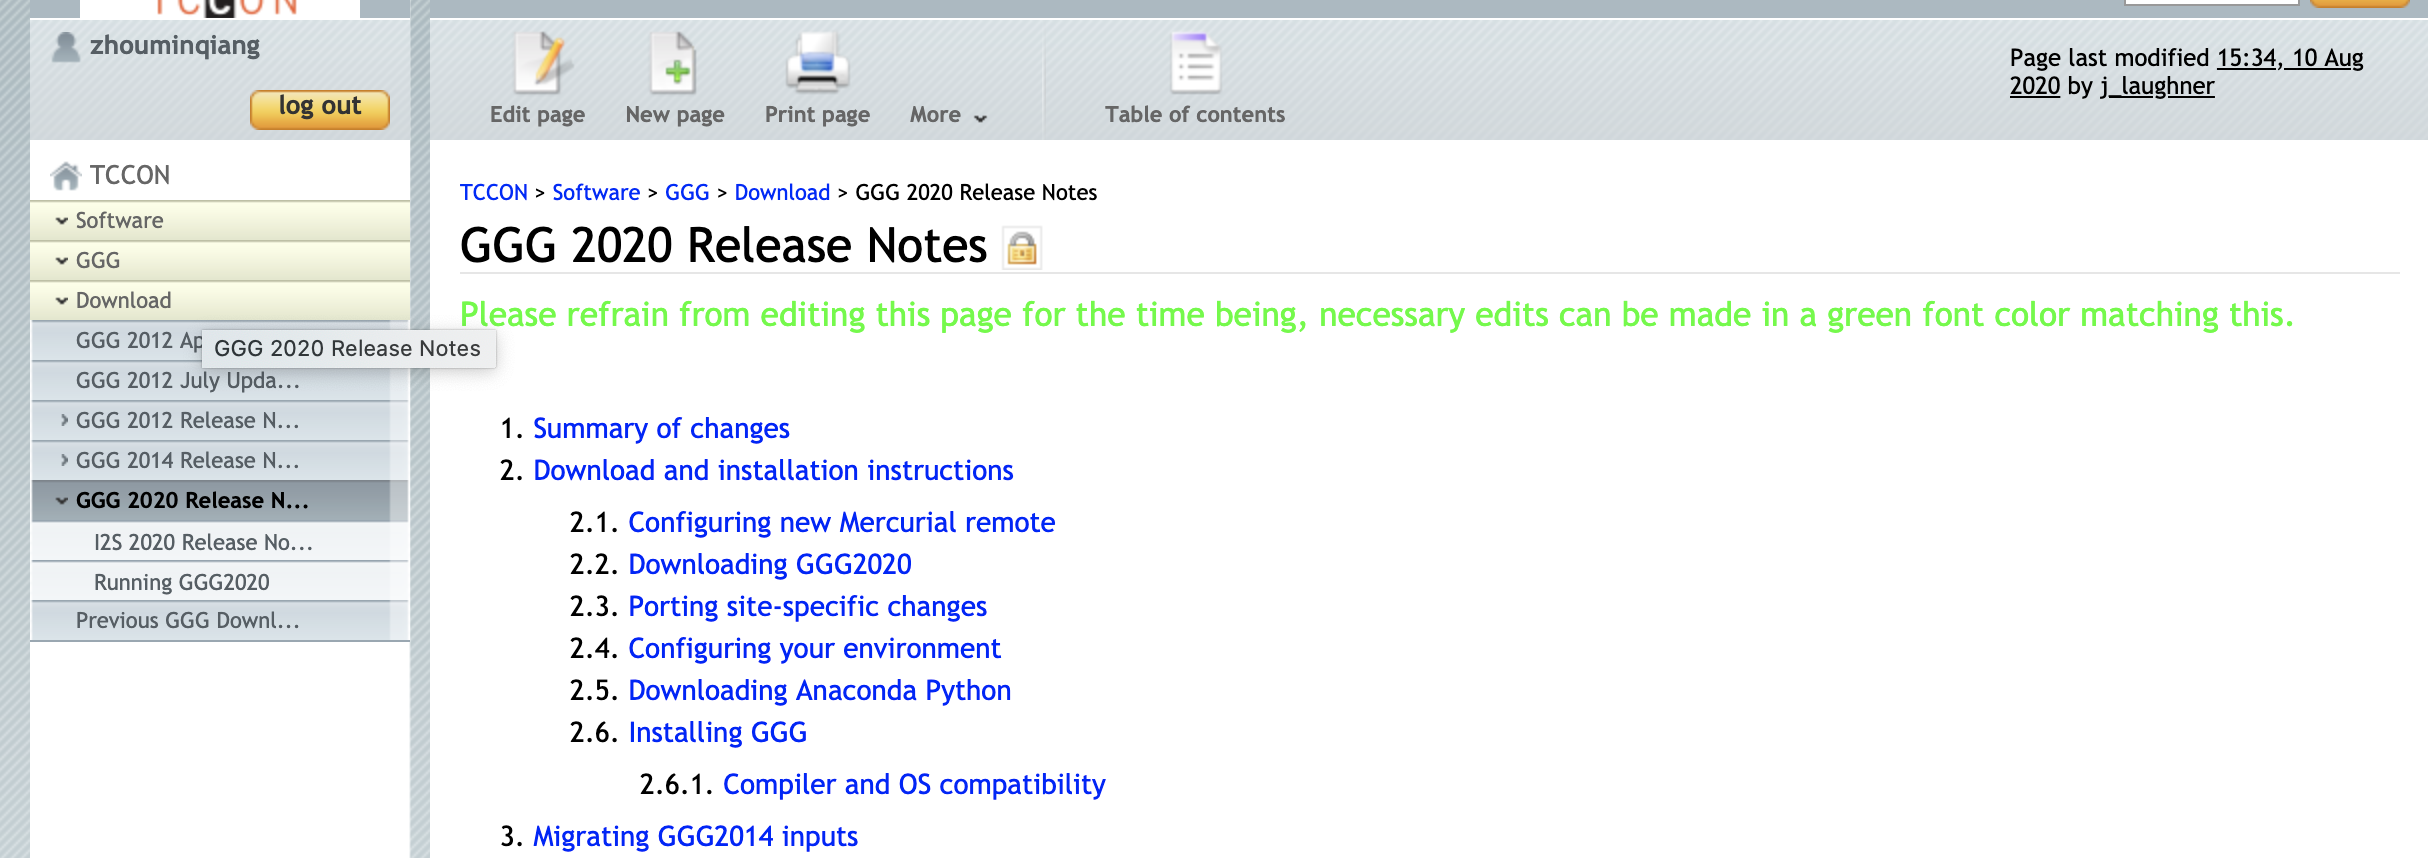
\includegraphics[width=1.0\textwidth]{./figure/tcconwiki.png} 
\caption{GGG2020 download.}
\end{center}
\end{figure}


\item[Steps] \hfill \\
STEP 1: cd \$GGGPATH/install  \\
STEP 2: ./master.sh 4  (you will crash, as you do not have the write to install the python lib in the default folder) \\
STEP 3: change the  install/clone\_netcdf\_writer.sh \\
(do not overwrite again as you do not download the tccon\_netcdf python code again; I already change the code in the ggg2020/install folder) \\
STEP 4: change the src/tccon\_netcdf 
(install the python lib to a user defined place: --prefix  )\\
STEP 5: add the prefix folder to install the python lib, for example, ggg2020/python\_tool/lib/python3.7/site-packages \\
STEP 6: cd \$GGGPATH/install  \\
Type ./master.sh 4\\
you need to input Y and N \\
then check the difference.out \\
the whole process will take about 20 mins\\


\item[Other notes]\hfill \\
1) GGGPATH should be GGGPATH=/bira-iasb/projects/FTIR/retrievals/operational/tools/ggg2020 instead of GGGPATH=/home/user/projects/FTIR/retrievals/operational/tools/ggg2020\\
2) for the conda environment, you might need to install some packages:\\
conda install -c conda-forge mercurial\\
conda install -c anaconda setuptools\\
3) in the src/gfit.f\\
change write(csfilename,'(a14,i6.6,a4)') 'check\_md5sums\_',pid,    -->     write(csfilename,'(a14,i7.7,a4)') 'check\_md5sums\_',pid,\\
in our system the getpid return 7 int instead of 6\\


\end{description}

\subsection{ggg3 at BIRA-IASB }
\label{download by git}
\begin{description}
\item[download by git]\hfill \\
make a folder, for example, in ftir\_op/python/. \\
git clone https://github.com/zmq814/ggg3\_bira.git \\
you will have ggg3\_bira folder where you have \\
\begin{figure}[h]
\begin{center}
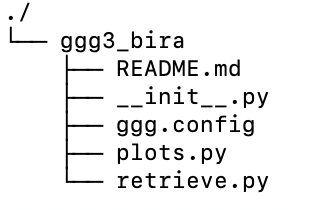
\includegraphics[width=0.5\textwidth]{./figure/ggg3.png} 
\caption{ggg3\_bira code.}
\end{center}
\end{figure}
\item[Run ggg3] \hfill \\
The code has been tested with the new PC, ada 1...5 using the 19g packages \\
I have define a m19p3geo in the .profile\\
Step1. in the terminal, INPUT m19p3geo \\
step2. in the python section, import ggg3\_bira.retrieve as r\\
step3. import datetime as dt\\
step4. stime = dt.datetime(),etime = dt.datetime(),instrument='bruker125@stdenis'\\
step5. r.main(instrument,stime,etime)\\

\end{description} 
 
%----------------------------------------------------------------------------------------


\end{document}